\documentclass{standalone}
\usepackage[dvipsnames,svgnames,x11names]{xcolor}
\usepackage{tikz}
\usepackage{pgfplots}
\pgfplotsset{compat = 1.12}
\usepackage{../thesismath}
\begin{document}
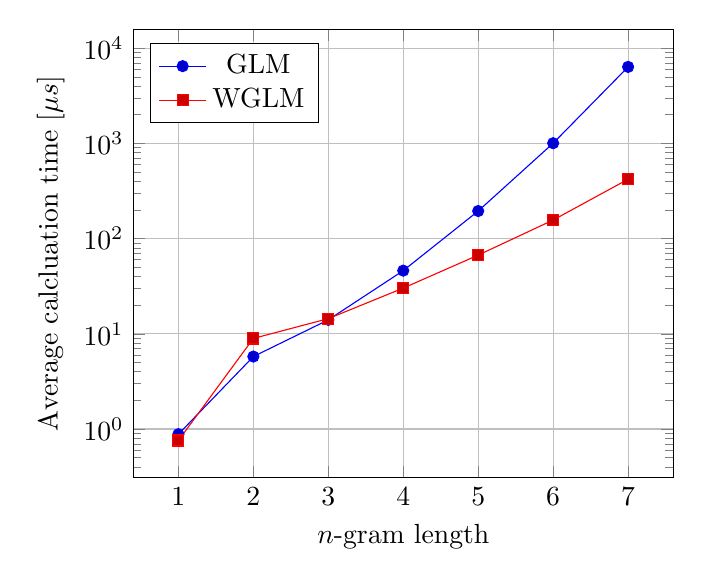
\begin{tikzpicture}[baseline]

\begin{axis}[
  xlabel = {$n$-gram length},
  ylabel = {Average calcluation time [${\mu}s$]},
  ymode = log,
  %yticklabel pos = right,
  minor y tick num = 4,
  grid = major,
  legend entries = {{GLM}, {WGLM}},
  legend pos = north west,
]

% GLM
\addplot table {
  n us
  1 0.883
  2 5.771
  3 14.022
  4 46.082
  5 194.878
  6 1004.226
  7 6355.396
};

% WGLM
\addplot table {
  n us
  1 0.758
  2 8.947
  3 14.436
  4 30.208
  5 67.092
  6 156.715
  7 420.214
};

\end{axis}

\end{tikzpicture}
\end{document}
